\chapter{Literature Survey}
\label{ch:litsurvey}
In this section, prior work in the field of image steganography and steganalysis are explored. This chapter is divided into five sections. The first section discusses popular steganographic implementations that are to be detected by the experimental setup described in the following chapter. The second section provides an overview of tools that implement steganography. Software tools that implement various approaches to steganalysis are described in the third section. The final two sections of this chapter are dedicated to describing theoretical and practical attacks on steganography respectively.
\section{Approaches to Image Steganography}
\label{sec:overview}
A large amount of literature exists on different methods to encode data in images. Early work in this area explore secure digital watermarking techniques for copyright enforcement which led to the creation of robust watermarking algorithms that were resilient to image manipulation. The use of similar techniques for secret communication using digital images followed thereafter. Freely available steganographic tools implement one or more of the following algorithms for embedding data in images. The data need not be restricted to text, it is possible to embed any other digital format into images. 
\subsection {Least Significant Bit image steganography}  LSB encoding is perhaps the most simple form of steganography. In this form of steganography, the image to be used can be represented as an array of RGB tuples with each colour value represented as a binary string. If the image is a 24 bit colour image, each colour value is represented by 8 bits as shown in \ref{eq:lsb}. The message to be encoded is usually compressed and encoded as a binary string. A simple algorithm would now begin encoding the data into the image starting from the first colour value representation and moving on until it has finished encoding the entire message. 
\begin{equation}
\label{eq:lsb}
\begin{split}
\text{\emph{Bits from image}}
\\
10110011\ 10001101\ 11111011 \\
10111000\ 10010100\ 01110111 \\
\\
\text{\emph{Bits to be encoded}}
\\
101100\\
\\
\text{\emph{Result, modified bits are shown in bold}}
\\
10110011\ 1000110\mathbf{0}\ 11111011 \\
1011100\mathbf{1}\ 10010100\ 0111011\mathbf{0} \\
\end{split}
\end{equation}
Variants of the LSB steganography algorithm may use random bits of the host image which can be dervied from a secret key. Visual changes caused to the image are minimal for 16bit/24bit colour images. If the colour depth is lower, a substantially large message (< 25\%) would cause degradation in image quality. 
\subsection{Frequency Domain Encoding} This is a slightly more sophisticated steganographic technique and is implemented in a number of tools like JSteg \cite{jsteg}. This scheme uses colour frequencies of the host image to hide data. The frequency distribution can be transformed into a ring structure by using a 2D Fast Fourier Transform (FFT). The FFT function, when applied to the image frequency distribution produces a ring like structure with the lower frequencies represented at the centre and the higher frequencies towards the edges. By converting a digital image into its constituent frequency distribution and subsequently using a 2D FFT function, it is possible to utilise the mid-range frequencies to encode data. The host image containing the steganographic message is retrieved using an inverse FFT that returns the image. Both LSB encoding and Frequency Domain Encoding require images that are approximately 3 times larger than the message to be encoded. Frequency Domain Encoding provides better protection against the discovery of the secret message when compared with Least Significant Bit encoding and is only marginally affected by file compression. 
\subsection{BPCS encoding} Bit-Plane Complexity Segmentation Based Embedding is a relatively new and potentially more effective way of data hiding.  A digital image can be segmented into a number of bitplanes of increasing complexity \cite{kawaguchi1998concept}. This segmentation divides the image into planes in such a way that each plane contributes some amount of detail to an image. The higher order planes contain the most detail and represent the features available in the image. The lower order planes contribute very little and appear as noise when viewed on their own.  For an image of size $n$ it is possible to use as much as $\frac{n}{2}$ of the image for hiding data provided that the image is sufficiently complex. For simpler images, any alteration to lower order bit planes that constitute the image would be readily evident.
\subsection{Image File Padding} This method of steganography does not require modifications to the colours of the image directly. Instead it relies on the fact that it is possible to pad an image towards the end with the secret. This is also not a very reliable scheme as padding a large amount of text into a relatively small image would cause the image file to be corrupted. It would, however, work reasonably well for small sized textual data (< 10\% of image size).
\begin{figure}[h!]
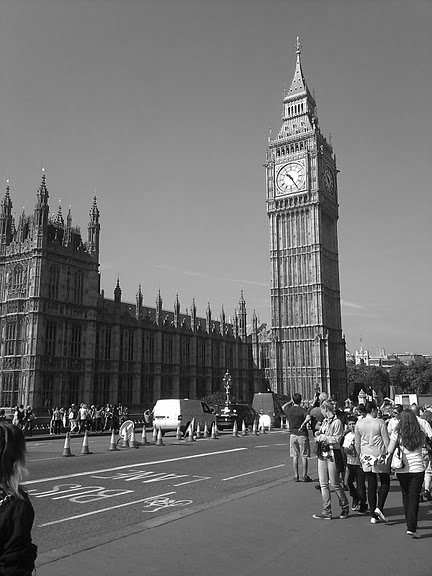
\includegraphics[scale=0.3]{embedded1}
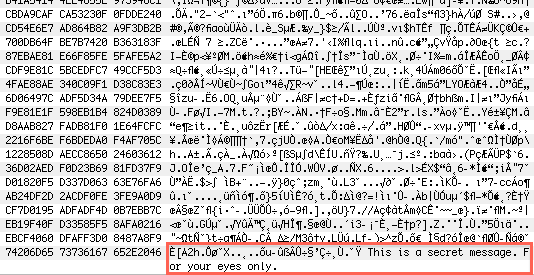
\includegraphics[scale=0.5]{embedded2}
\caption{\emph{The image on the left contains text embedded at the end of the image file. The embedded data can be viewed using a hex editing tool as shown on the right}}
\label{fig:embedded}
\end{figure} 

\section{Image Steganography Tools}
\label{sec:tools}
In this section an overview of popular steganographic tools is presented. It was found that while a number of tools are available for steganography, many of them share similar algorithms to encode data in digital files.  The tools are evaluated on the basis of their availability, the operating system platforms they support and the algorithms implemented by them. Non free tools were not evaluated as part of the project. 
\subsection{EzStego}
EzStego \cite{ezstego} is a free steganographic tool created by Romana Machado  implemented in Java and is available for the most common operating systems (Linux,Windows, MacOS). The software appears to be no longer maintained but copies of it are mirrored in other locations of the web. The steganograms produced by EzStego have been extensively studied by a number of authors  \cite{westfeld2000attacks, farid2002detecting}. It is most susceptible to the visual attack as it relies of Least Significant Bit encoding (LSB) to hide data in a GIF file. 
\subsection{S-Tools}
S-Tools \cite{stools} are a collection of steganographic tools that allow for data hiding in a number of digital file formats. Supported formats include WAV, GIF and BMP files. It is not possible to use a JPEG file as a medium for steganographic data using this software.  S-Tools also allows the user to choose between DES, Triple DES, IDEA and MDC encryption algorithms. In order to recover data from S-Tools created steganograms,  the user is required to know the passphrase that was used as the key to encrypt the data and the encryption algorithm used.  S-Tools is available for Windows and UNIX like operating systems.
\subsection{JSteg} 
JSteg \cite{jsteg} is a steganographic tool that allows a user to embed messages in JPEG files, the message size is limited to roughly 12\% of the image size. It has been extensively studied by a number of authors including Westfeld and Goljan. The image medium used is JPEG, which is a lossy image compression algorithm. Owing to this images containing data encoded with JSteg are immune to traditional visual attacks unlike EzStego, which requires an uncompressed Bitmap image as the medium. Due to the use of JPEG as an the medium, it is not possible to reliably isolate data that is encoded in the least significant bit field and prove the existence of steganography. Steganograms produced by JSteg are, however, still vulnerable to statistical attacks. JSteg is written in C and is available for Windows and UNIX like operating systems.
\subsection{JPHide and Seek}
JPHide and Seek \cite{jphide} was written by Alan Latham and it is exclusively designed to hide data in JPEG images. It's primary design goal is providing plausible deniability \emph{i.e.} it should be difficult or impossible to prove that a particular image contains steganographic data. This goal is acheived if the message length is less than 15\% of the size of the image and the image contains significant detail (\emph{e.g.} a picture of a forest with a river). Separate versions for Windows and Linux are available.
 \subsection{F5}
 The F5 algorithm \cite{westfeld2001f5} was created by Westfeld to provide a steganographic solution that was resilient to both visual and statistical attacks. This is made possible by the design of the F5 algorithm that uses matrix encoding for data and uses permutation techniques to distribute the data throughout the steganographic medium. Unlike LSB based steganography software like JSteg and S-Tools, F5 encodes data by manipulating the DCT coefficients in a JPEG image. 
 \subsection{StegMark}
 StegMark \cite{stegmark} is a commercial software product developed by DataMark Technologies. It is not strictly designed for steganographic communication; instead this software implements digital watermarking using steganography. Digital watermarking can be used to enforce digital content ownership and prevent plagiarism of images or other digital media. It can, however, be used to communicate covertly as it provides an SDK for creating steganography tools. StegMark is available for Windows as a C++ SDK.
 \subsection{Stepic \& ESFS}
 Stepic \cite{stepnic} is a relatively new steganography tool written by Lenny Domnitser in Python. The steganography implementation appears to be pedagogical as it only provides data hiding by using LSB encoding. Another project, the Encrypted Steganographic Filesystem (ESFS) \cite{esfs}, has adapted Stepic to provide a File System in User Space (FUSE) based filesystem for Linux. StegFS also provides an additional security by encrypting the data using AES with a 256 bit key. It is a proof of concept implementation and the author claims that the performance is relatively poor. Stepic is available as open source software for both Windows and UNIX like operating systems while ESFS requires Linux and Python with the cryptographic toolkit (pycrypto) installed.
 \subsection{Digital Picture Envelope}
 Digital Picture Envelope is the result of research \cite{kawaguchi1998concept} in the area of Bit Plane Complexity Steganography(BPCS). This method of steganography is radically different from the other implementations that rely on LSB encoding to hide data. The Digital Picture Envelope converts the host image into a number of bit planes, each plane constitutes part of the image. The most complex planes can be used as information carriers as changes to it cannot be perceived by the human eye.  An added advantage is that unlike other steganographic mechanisms, BPCS \emph{alters} the actual image instead of appending to it thereby ensuring that the steganogram is the same size as the original image. Additionally, up to 50\% of the image can be used to store the data. Digital Picture Envelope is available in binary format for Windows systems only. 
 
\section{Image Steganalysis Tools}
\label{sec:steganalysistools}
In this section we discuss a number of tools that provide steganalysis features. There are very few free tools that implement all steganalysis attacks.Proprietary tools rely heavily on image hashsets and other proprietary detection methods that are not disclosed. For the purpose of this project it wasnecessary to identify a set of tools that will provide a universal system for steganalysis \emph{i.e.} the tools should be able to prove the existence of steganography in a given image. Some of the tools that implement steganalysis are:
\subsection{Outguess}  Outguess \cite{outguess} ships as a package that provides steganography tools as well steganalysis tools. It implements custom detection routines for popular steganography algorithms like JSteg, F5 and JPHide. It also provides the command line tools stegdetect and stegbreak, the former implements steganography detection while the latter provides a tool that attempts to extract data from a steganogram using brute force and dictionary attack methods. It is available as open source software with source and binaries for all platforms. 
\subsection{Virtual Steganography Laboratory} VSL \cite{wegrzyn2009} is provided as an open source steganography and steganalysis Java software package. It implements F5 \cite{westfeld2001f5}, Karhunen-Loeve Transform \cite{stanescu2007digital} and Least Significant Bit steganography. It was designed as an educational tool and all steganography/steganalysis functions are written as separate modules. It is still under active development and the author intends to add more modules in the future.
\subsection{Gargoyle} Gargoyle \cite{gargoyle} is a commercial malware removal product that ships with a proprietary database of hashsets. These hashsets provide a method of identifying steganographic content by checking for ``signatures'' left by steganographic software. The software package is available for Windows and is designed for forensic investigators.
\subsection{EnCase}Another commercial software product \cite{encase} that provides various  computer forensic features. It has features that allow for steganographic detection. Encase runs on Windows and employes signature based detection to check for the presence of steganography.
\subsection{AccessData Forensic Toolkit} This commercial tool allows for the identification of steganography based on proprietary hashsets \cite{ftk}. Like Gargoyle and Encase, it can only identify the presence of steganography in files by means of hash analysis. It is limited to identify a finite number of specific steganography algorithms. 
 
The availability of free image steganalysis tools is limited as compared to the numerous options available for image steganography. A few steganography suites, like Outguess \cite{outguess} provide a combined steganography/steganalysis software suite. Commercially available tools like Encase, provide steganalysis as part of a digital forensics toolkit.  

\section{Previous Work in Steganalysis}
\label{sec:theory}
Pfitzmann and Westfield \cite{westfeld2000attacks} describe two methods for analysing images for steganographic content. The first method is the use of visual techniques to identify whether an image could contain steganographic content.  This is done by first extracting the potential message bits (\emph{i.e.} bits of the image that may have been used for hiding data). The other bits of the image that are non steganographic are removed and only potential message bits are illustrated using black and white as shown in Figure \ref{fig:visualattacks}. This allows an observer to see that the image may contain data.
\begin{figure}[h!]
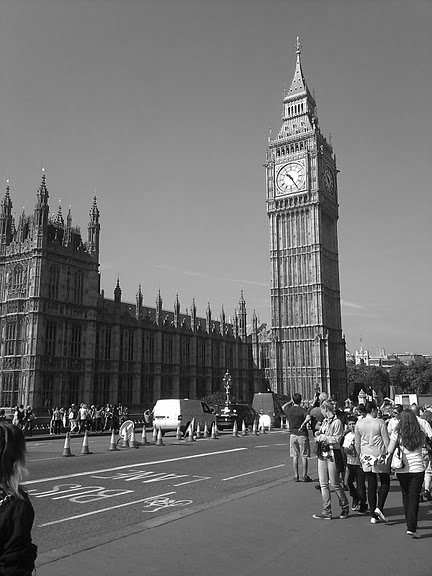
\includegraphics[scale=0.5]{visual1}
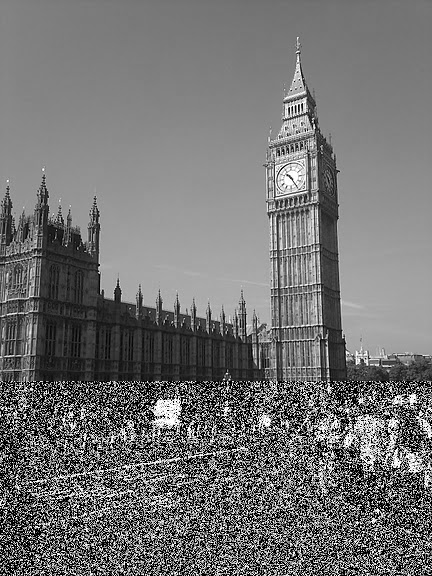
\includegraphics[scale=0.5]{visual2}
\caption{\emph{The image on the left contains steganographic data embedded in the lower half of the image. Visual attacks involve extracting and highlighting the areas of the image that could contain steganographic material as shown in the figure on the right}}
\label{fig:visualattacks}
\end{figure} 

\par The second method utilises the $\chi^{2}$ statistical test to determine if the image contains steganographic content. In this method,  the theoretical expected frequency distribution of pixels in an image is compared with the actual frequency distribution of the pixels in the steganographic image. A deviation between these values indicates the presence of a steganographic message. This is possible as the tools used for creating the steganographic image incorrectly assume that the Least Significant Bits are random and can be overwritten to hide message. The authors claim that statistical tests provide a much higher accuracy than visual attacks and should be used when possible. 
\par Building on the works of Pfitzmann et al  \cite{westfeld2000attacks}, Fridrich and Goljan \cite{fridrich2002practical} present a collection of qualitative methods for practical steganalysis. The authors extend the statistical analysis described by both Pfitzmann and Provos to include the spatial arrangement of pixels in a steganographic image referred to as ``Dual Statistical attacks''.  
\par The JPEG compatibility attack described by Goljan et al relies on finding non compatible JPEG artefacts in images. The image to be analysed is divided into  8x8 pixel blocks and the algorithm attempts to locate blocks that would not ordinarily be produced by the JPEG compression algorithm.
\par A universal, ``meta'' steganalysis approach from Farid  \cite{farid2002detecting} is also described by the author, which attempts to detect the presence of steganography rather than being a targeted approach towards a specific steganographic algorithm.  This approach utilises higher order statistical modelling that provides a generic approach to detect the presence of steganographic content in images. Farid's experimental setup consists of three types of support vector machines (SVMs). A support vector machine is a data classifier with a very high degree of accuracy \cite{noble2006support}. The kernel parameters for the support vector machine were tuned as to provide a very low (1.0\%) false positive rate. They were then trained with a library of GIF, JPEG and TIFF images. The trained SVMs were used to classify a large number of mixed (steganographic and non steganographic) images. It was discovered that with a low false positive rate, a non-linear SVM was able to accurately classify 90.2\% of steganographic images of size $160\times160$ pixels correctly with a false negative rate of 9.8\%.
\par It is to be noted that all studies mentioned in this section attempt to analyse steganographic images that were specifically created for the purposes of the experiments starting with clean stock images. Images obtained from the internet were not used as part of the study for any of these experiments.
\section{Practical Attacks on Image Steganography}
\label{sec:practical}
An exhaustive study carried out in 2001 by Provos and Honeyman \cite{provos2001detecting} analysed over 2 million images downloaded from eBay auctions using stegdetect, a tool created for detecting multiple kinds of steganography. Images that were classified as being suspicious were subjected to a dictionary attack to attempt recovery of the message.
\par Their results did not find any significant use of steganography in images that were posted as part of the auctions. However they do not discount the possibility that the images they analysed were using steganographic techniques that were not not detectable by the methods employed by them.
\par For the few thousand images that were discovered to have been marked as suspicious by their setup, it was not possible to recover any of the messages embedded in them.  They speculate that it could have been due the use of a strong password to encrypt the message stored in the images.

\section{Summary of Literature Review}
\label{sec:summarybg}
In this chapter, important studies in the areas of steganography and steganalysis relevant to this project have been covered. A selection of tools that implement steganography and steganalysis were also discussed.  Deriving from previous works in this area, an experimental setup designed for the detection of image steganography from a random sample of freely available images which is discussed in detail in the following chapter.
